\chapter{Implementacja systemu}


\section{Kadrowanie twarzy}

Zdjęcia, które zostaną przesłane na serwer, należy w pierwszej kolejności odpowiednio przygotować.
W tym celu została wykorzystana wcześniej wspomniana biblioteka PILLOW,
która ma za zadanie wykonać przekształcenie otrzymanego pliku do tablicy pikseli.
Otrzymana tablica następnie trafia do sieci MTCNN, która zwraca informacje na temat wykrytych twarzy,
po czym następuje wycinanie fragmentu zdjęcia przedstawiającego samą twarz.
Jeżeli nie zostaną znalezione żadne twarze, funkcja rzuci odpowiednim błędem.


\section{Generowanie wektora cech}

Po wykadrowaniu twarzy, kolejnym krokiem jest wygenerowanie wektora cech.
Odpowiednio przygotowana wcześniej tablica pikseli jest standaryzowana,
ponieważ wymaga tego używana implementacja architektury FaceNet, a następnie wykonywana jest predykcja.
Jako wynik działa funkcji zwracany jest opisany wcześniej wektor cech.


\pagebreak


\section{Ocena podobieństwa twarzy}

FaceNet został nauczony tak, aby mapować zdjęcia twarzy do zwartej przestrzeni euklidesowej,
w której odległości pomiędzy punktami bezpośrednio odpowiadają mierze podobieństwa twarzy.
Oznacza to, że jeżeli odległość pomiędzy dwoma punktami w przestrzeni
jest względnie mała, to jest wysoce prawdopodobne, że zdjęcia twarzy przedstawiają tę samą osobę.
Mając to na uwadze, można znaleźć odległość, poniżej której zostałoby uznane, że zdjęcia
przedstawiają tę samą osobę (rysunek~\ref{fig:szukanie_progu}).

\begin{figure}[H]
    \centering
    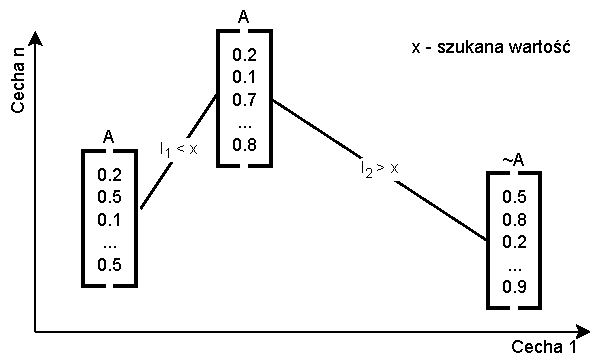
\includegraphics[width=1\textwidth]{./images/szukanie_progu}
    \caption{ Wizualizacja szukanego progu podobieństwa. Jeżeli odległość pomiędzy punktami jest
    zmniejsza niż wartość ``x'' to program powinien uznać, że wektory opisują tę samą osobę. }
    \customsource
    \label{fig:szukanie_progu}
\end{figure}

\pagebreak

\subsection{Poszukiwanie odległości}

Do poszukiwania wartości progu zostało wykorzystanych około \num{5000} losowo wybranych zdjęć,
przedstawiających około \num{500} różnych osób, po około \num{10} zdjęć na osobę,
z bazy CelebA~\cite{liu2015faceattributes}.
Na każdym zdjęciu zostało następnie wykonane kadrowanie twarzy oraz generowanie wektora cech.
Ostatnim elementem było zbadanie odległości pomiędzy wszystkimi wektorami tych samych oraz różnych osób.
Całość badania można podsumować w następujących krokach:
\begin{enumerate}
    \item wygenerowania wektora cech dla każdego z dostępnych zdjęć,
    \item wybranie wektora cech ze zbioru,
    \item zmierzenie odległości pomiędzy wybranym wektorem i wszystkimi pozostałymi wektorami z uwzględnieniem,
    czy wektory cech reprezentują tę samą osobę, czy dwie różne osoby,
    \item powrót do kroku drugiego do momentu, aż zostaną zbadane wszystkie odgległości (każdy z każdym).
\end{enumerate}
Wyniki przeprowadzonych kroków zostały przedstawione w postaci histogramów na rysunku~\ref{fig:porownanie_histogramow_odleglosci}.

\begin{figure}[H]
    \centering
    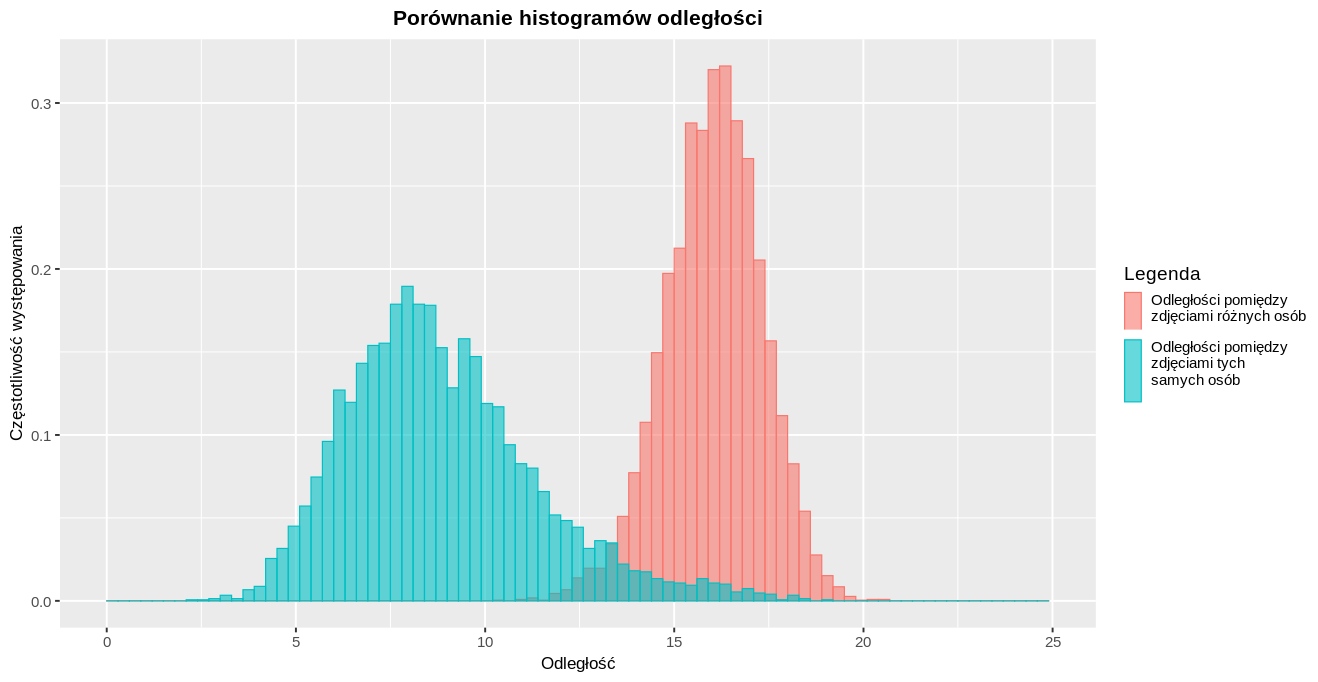
\includegraphics[width=1\textwidth]{./images/porownanie_histogramow_odleglosci}
    \caption{ Porównanie histogramów odległości pomiędzy wektorami twarzy tych samych oraz różnych osób }
    \customsource
    \label{fig:porownanie_histogramow_odleglosci}
\end{figure}

\pagebreak

Na podstawie histogramów (rysunek~\ref{fig:porownanie_histogramow_odleglosci}) można zauważyć,
że nie istnieje taka wartość, która jest w stanie odseparować przedstawione zbiory.
Należy jednak zwrócić uwagę na to, że w badaniu zostały wzięte odległości pomiędzy \textbf{każdym} zdjęciem z grupy.
Przy ocenie podobieństwa pomiędzy twarzami nie ma potrzeby patrzenia na odległości na całym zbiorze zdjęć.
Po wygenerowaniu wektora cech dla danego zdjęcia interesujący jest tylko ten wektor, który
leży \textbf{najbliżej} wygenerowanego (rysunek~\ref{fig:najmniejsze}).

\begin{figure}[H]
    \centering
    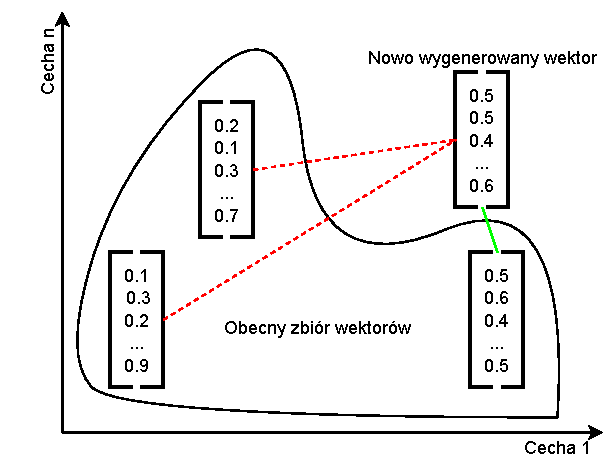
\includegraphics[width=1\textwidth]{./images/dlaczego_najmniejsze}
    \caption{ Schemat obrazujący najbliższą odległość pomiędzy nowym wektorem a zbiorem.
    Na czerwono zostały oznaczone odległości do dalszych wektorów. Na zielono została oznaczona odległość
    do najbliższego wektora i to względem niego system powinien oceniać podobieństwo.
    }
    \customsource
    \label{fig:najmniejsze}
\end{figure}

\pagebreak

Biorą pod uwagę opisany problem, wyżej opisane badanie zostało powtórzone, jednak w tym przypadku
zostały zapisane tylko odległość do najbliższego wektora.
Całość zatem można podsumować w następujących krokach:
\begin{enumerate}
    \item wygenerowania wektora cech dla każdego z dostępnych zdjęć,
    \item wybranie wektora cech ze zbioru,
    \item znalezienie wektora, który leży najbliżej względem wybranego i zapisanie odległości
    z uwzględnieniem czy znaleziony wektor reprezentuje tę samą osobę,
    \item powrót do kroku drugiego do momentu, aż zostaną wybrane wszystkie wektory.
\end{enumerate}
Wyniki powtórzonego badania zostały ponownie przedstawione w postaci
histogramów na rysunku~\ref{fig:wykres_najmniejszych_odleglosc_wspolny}.

\begin{figure}[H]
    \centering
    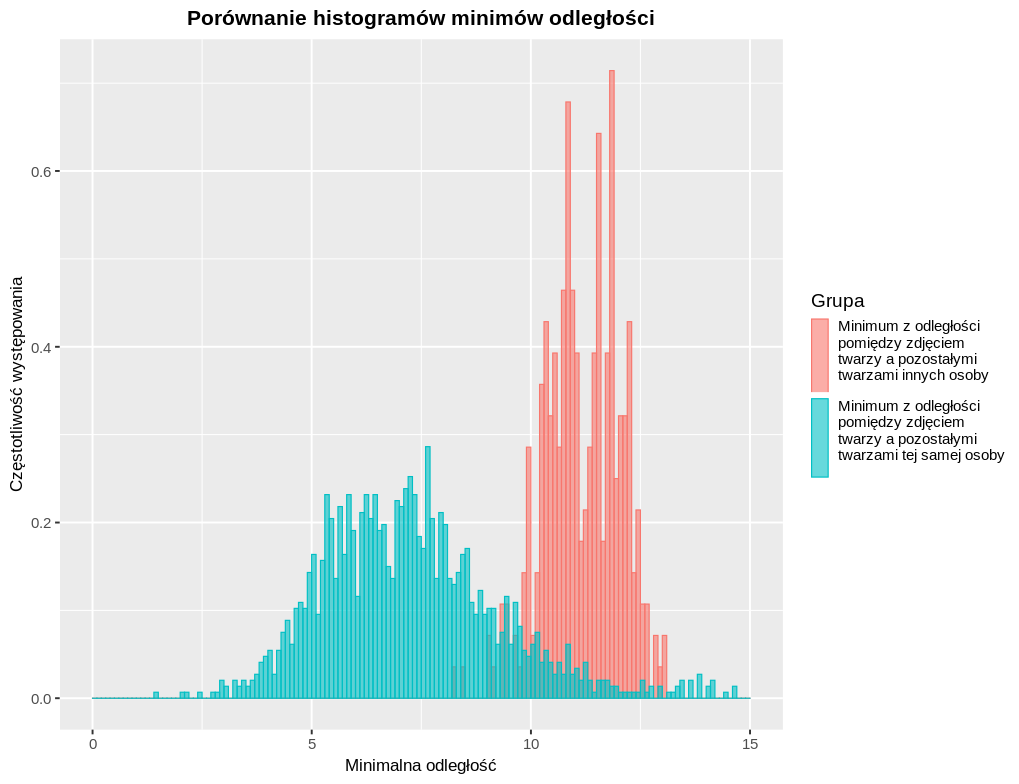
\includegraphics[width=1\textwidth]{images/wykres_najmniejszych_odleglosc_wspolny}
    \caption{
        Porównanie histogramów najmniejszych odległości pomiędzy
        zdjęciami twarzy tych samych oraz różnych osób.
    }
    \customsource
    \label{fig:wykres_najmniejszych_odleglosc_wspolny}
\end{figure}

\pagebreak

Z histogramów (rysunek~\ref{fig:wykres_najmniejszych_odleglosc_wspolny}) wykonanego badania również wynika,
że nie istnieje taka wartość, która będzie w stanie odseparować przedstawione zbiory.
Konsekwencją tego jest, że dla dowolnego ``x'' będą istnieć przypadki, dla których
zdjęcia błędnie zostaną uznane, że przedstawiają tę samą osobę.
Należy zatem znaleźć taką wartość ``x'', dla której funkcja oceniająca, czy wektory
dotyczą tej samej osoby, będzie miała największą skuteczność.
Przedział, w jakim należy spodziewać się największej trafności,
powinien (jak wynika z rysunku~\ref{fig:wykres_najmniejszych_odleglosc_wspolny})
znaleźć się w przedziale od \num{8} do \num{12}, ponieważ na tym odcinku
oba histogramy pokrywają się na największym obszarze.

\subsection{Odległość o największej skuteczności}

W celu sprawdzania dla jakiego ``x'' ocena podobieństwa osiągnie maksymalną wartość,
wspomniany wcześniej zbiór zdjęć, został podzielony na dwie grupy.
Do pierwszej grupy trafiły zdjęcia, które zasiliły system i stanowiły bazę
w weryfikowaniu, czy nowe zdjęcie, które zostanie dostarczone,
zostanie uznane za podobne do jakiegoś zdjęcia twarzy, które znajduje się już w systemie.
Do drugiej grupy trafiły zdjęcia, które podlegały ocenie przez system, czy owo zdjęcie jest znane systemowi.
Dokładny podział zdjęć został przedstawiony na rysunku~\ref{fig:podzial_zdjec}.

\begin{figure}[H]
    \centering
    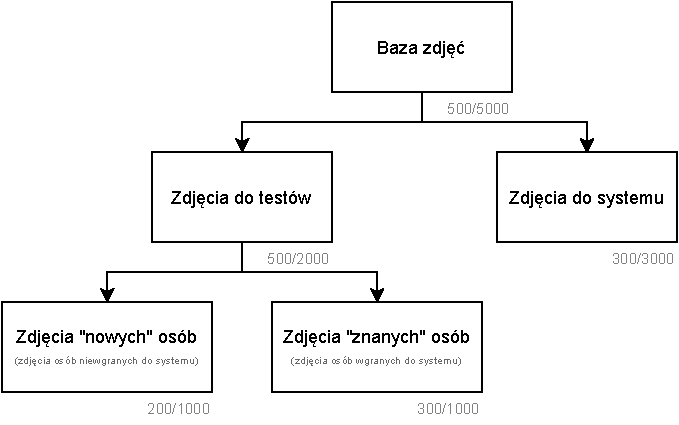
\includegraphics[width=1\textwidth]{images/podzial_zdjec}
    \caption{
        Podział zdjęć na grupy. Obok każdej z grupy widnieje liczba osób oraz suma
        wszystkich zdjęć należąca do owej grupy.
    }
    \customsource
    \label{fig:podzial_zdjec}
\end{figure}

Po podzieleniu zdjęć na grupy kolejnym krokiem jest zbadanie trafności oceny podobieństwa dla poszczególnych
progów z zakresu od \num{8} do \num{12}.
Zakres ten będzie badany z dokładnością do \num{0.1}.
Kroki, jakie zostały wykonane w badaniu, są następujące:

\begin{enumerate}
    \item wygenerowanie wektora cech dla wszystkich zdjęć z każdej grupy,
    \item wgranie wygenerowanych wektorów z grupy ``Zdjęcia do systemu'' do systemu,
    \item pobranie zdjęć z grupy ``Zdjęcia nowych osób'' i przepuszczenie ich przez
    funkcję oceniająca podobieństwo na podstawie wgranych zdjęć do systemu dla danego ``x'',
    \item powtórzenie kroku trzeciego dla zdjęć z grupy ``Zdjęcia znanych osób'',
    \item potwórzenie kroku trzeciego oraz czwartek dla nowego parametru ``x''.
\end{enumerate}

Dla kroku trzeciego, przy założeniu, że skuteczność oceny podobieństwa była by stuprocentowa, funkcja
powinna zwrócić zawsze wartość \textit{False}, ponieważ \textbf{żadna} z osób przedstawiona
na zdjęciach z grupy ``Zdjęcia nowych osób'' nie znajduje się w systemie.
Dla kroku czwartego, w przeciwieństwie do kroku trzeciego, funkcja ta powinna
zawsze zwrócić \textit{True}, ponieważ \textbf{każda}
osoba przedstawiona na zdjęciu z grupy ``Zdjęcia znanych osób'' znajduje się w systemie.
Niestety z przeprowadzonych wcześniej badań (rysunek~\ref{fig:wykres_najmniejszych_odleglosc_wspolny}) wynika,
że taki scenariusz nie jest możliwy i z tego powodu należy znaleźć taką wartość parametru ``x'',
dla którego trafność walidatora oceniającego podobieństwo będzie maksymalne.

Wyniki opisanego wcześniej badania zostały przedstawione na rysunku~\ref{fig:tranosc_walidatora_per_prog}.
Na jego podstawie można zauważyć, że trafność walidatora
rośnie wraz ze wzrostem wartości progu aż do momentu osiągnięcia
przez ``x'' wartości \num{10.2} po czym nastepuje spadek.
Dla wartości \textbf{10.2} trafność funkcji została oceniona na poziomie \textbf{92.3\%}.
Obliczony wartość oznacza, że jeżeli odległość pomiędzy dwoma wektorami, które leżą najbliżej siebie,
jest mniejsza niż \num{10.2} to system uzna, że owe wektory dotyczą tej samej osoby,
przez co proces będzie kontynuowany.
W przeciwnym wypadku zostanie rzucony błąd z informacją, że osoba przedstawiona na zdjęciu,
która podlega weryfikacji, nie jest znana systemowi.

\begin{figure}[]
    \centering
    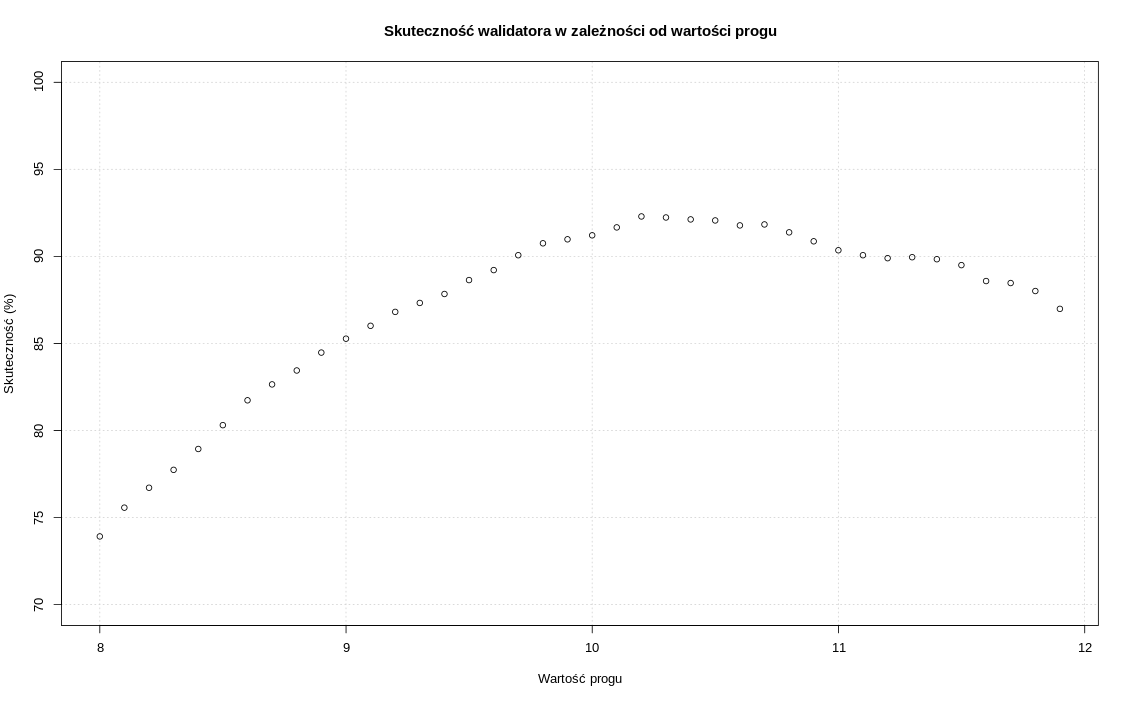
\includegraphics[width=1\textwidth]{images/trafnosc_walidator_a_prog}
    \caption{ Trafność walidatora w zależności od wartości progu (parametru ``x'') }
    \customsource
    \label{fig:tranosc_walidatora_per_prog}
\end{figure}

\pagebreak


\section{Klasyfikator}

Ostatnim krokiem w procesie działającym po stronie serwera (rysunek~\ref{fig:schemat_blokowy_systemu})
jest wykonanie klasyfikacji.
Na tym etapie wiadome już jest, że wektor cech, który trafił do klasyfikatora, reprezentuje osobę,
która jest znana systemowi.
Jest to bardzo istotna informacja, ponieważ w przeciwnym wypadku klasyfikator
mógłby dokonać klasyfikacji pomimo tego, że dana klasa (w tym wypadku osoba) nie istnieje w systemie,
co oznaczałoby zawsze błędną klasyfikację.

Do wykonywania klasyfikacji został wykorzystany klasyfikator SVM z liniowym jądrem z parametrem $C$ równym $1.0$.
Jego trafność na opisanym wcześniej zbiorze (rysunek~\ref{fig:podzial_zdjec}) wyniosła \textbf{96.1\%}.
Z powodu tak wysokiej trafności nie były testowane inne klasyfikatory.
Implementacja klasyfikatora SVM została zaczerpnięta z biblioteki \textit{sklearn}~\cite{sklearn_api}.


\section{Strona internetowa}

Zaprojektowana strona internetowa składa z prostego formularza.
Na stronie został umieszczony przycisk, który umożliwia wybranie zdjęć z dysku urządzenia klienta.
Po wybraniu zdjęcia pojawi się jego podgląd, po czym plik jest wysyłany na serwer.
Po uzyskaniu odpowiedzi z serwera zostanie wyświetlony otrzymany komunikat.
Wygląd strony zostaw przedstawiony na zdjęciu~\ref{fig:ja}.

\begin{figure}[H]
    \centering
    \includegraphicswithborder[width=1\textwidth]{images/wyglad_frontowa_aplikacji}
    \caption{Wygląd strony internetowej po wybraniu zdjęcia z dysku i uzyskaniu odpowiedzi z serwera}
    \customsource
    \label{fig:ja}
\end{figure}
